
\documentclass[annual]{acmsiggraph}
\usepackage{relsize} 

\usepackage{amsmath} 

\usepackage{algorithm} 

\usepackage[noend]{algorithmic}

\usepackage{listings}

\lstset{language=HTML}

\TOGonlineid{163}

\TOGvolume{}

\TOGnumber{} 

\TOGarticleDOI{} 

\TOGprojectURL{aw204.host.cs.st-andrews.ac.uk/camgaze.js} 

\TOGvideoURL{} 

\TOGdataURL{} 

\TOGcodeURL{}

\newcommand{\Acronym}[1]{\ensuremath{{\small{\texttt{#1}}}}}
\newcommand{\Name}{\Acronym{Camgaze.js}} \newcommand{\False}{\Constant{false}}
\newcommand{\True}{\Constant{true}}
\newcommand{\Symbol}[1]{\ensuremath{\mathcal{#1}}}
\newcommand{\Function}[1]{\ensuremath{{\small \textsc{#1}}}}
\newcommand{\Constant}[1]{\ensuremath{\small{\texttt{#1}}}}
\newcommand{\Var}[1]{\ensuremath{{\small{\textsl{#1}}}}}
\newcommand{\argmin}[1]{\underset{#1}{\operatorname{arg}\,\operatorname{min}}\;}

\title{Camgaze.js: Browser-based Eye Tracking and Gaze Prediction using
JavaScript}

\author{Alex Wallar \thanks{email: aw204@st-andrews.ac.uk} \\ Aleksejs Sazonovs
\thanks{email: as245@st-andrews.ac.uk} \\ University of St Andrews \and Patrick
Flynn \thanks{email: flynn@nd.edu} \\ Christian Poellabauer \thanks{email:
cpoellab@nd.edu} \\ University of Notre Dame}

\pdfauthor{Alex Wallar} 

\date{\today}

\begin{document}

\maketitle

\begin{abstract}

Eye tracking is a difficult problem that is usually solved using specialised
hardware and therefore has limited availability due to cost and deployment
difficulties. We describe $\Name$ – a client-side Javascript library that is
able to measure the point of gaze using only commodity optical cameras without
relying on any external application installed besides a web-browser. We conduct
experiments using $\Name$ to show the usability of such a system.  We also
discuss the challenges and applications of using an in-browser eye tracking
system. Since the described eye tracker works inside the browser without any
additional installation setup, it provides a solution to a larger deployment of
eye tracking systems.

\end{abstract}

\section{Introduction}

Eye tracking is a challenging problem, that has been attempted to be solved
since the 19th century \cite{Ahrens1891}. Currently, it is mostly viewed as a
problem in Computer Vision. The majority of eye tracking solutions available on
the market today are a combination of software and specialised hardware. The
principles behind hardware varies greatly: it ranges from head-mounted cameras
to lenses with integrated coils. It is believed that the state of the art
solutions can allow accuracy up to NN\% {link}. Despite that, carrying out eye
tracking experiments remains an issue – it is expensive, requires complicated
deployment and calibration and, in most cases, has to be carried out in a
controlled environment.

In the recent years, it has been shown \cite{SanAgustin2009}\cite{Sewell2010}
that it is possible to use commodity cameras, often built into modern
computers to perform eye tracking with promising quality. Deployment of such
systems is relatively simple, but in the described cases it is tied to specific
computer platforms \cite{holland2012eye}.

Web applications are “rich” websites that are able to run without external
plugins inside the browser. Recently, the web-browsers have evolved to adapt to
the market’s requirements – new technologies have risen, allowing web
application to be increasingly interactive. For example, WebRTC (Web Real-Time
Communication) is an API that aims to enable in-browser audio and video
communication. As of September 2013, WebRTC is supported in the stable versions
of Google Chrome and Mozilla Firefox. A recent report
\cite{DisruptiveAnalysis2013}, claims that by 2016 there will be
3 billion capable devices and 1 billion individual users of WebRTC-enabled
devices.

We describe $\Name$ -- a Javascript library that uses WebRTC to obtain the
video from built-in or USB cameras and measures the point of gaze. We believe
that it can be deployed in a wide range of applications such as website
interface analytics and concussion testing as well as interactive input.


\section{Challenges}

Running eye tracking on a wide range of hardware creates additional challenges.
The cameras that are built-in (or supplied with) consumer devices vary greatly:
there is no standard resolution, color profile, brightness level or physical
position. Currently, WebRTC provides very limited options for changing any of
the parameters of the camera that is providing a stream. This problem can be
partially addressed by defining individual profiles for a variety of popular
devices. The identification of the device is not a trivial task by itself, but
services like DeviceAtlas \cite{DeviceAtlas2013} solve it by looking at a
variety of factors, such as browser’s User Agent and screen resolution.
Unfortunately, this approach would be mostly applicable for handheld devices
and not commodity PCs.

The client-side Javascript environment in which $\Name$ runs in sets some
constraints. As of September 2013, we believe that there is lack of
comprehensive Computer Vision library implemented in Javascript. There is
currently no “simple” way to port native C/C++ code, which are languages in
which popular libraries such as OpenCV are written in. Projects like Emscripten
are making early attempts to allow translation of LLVM bitcode code to
Javascript, potentially allowing to port some of the well-established Computer
Vision libraries to Javascript in the future. For now, we had to create a
custom implementation of {ALEX} to use in $\Name$.

Despite some of the described difficulties, the authors of this paper believe
that a combination of Javascript and WebRTC is a reasonable technological stack
in order to implement an eye tracking solution, suitable for large scale
deployment.


\section{Implementation}

$\Name$ goes through three steps in order to predict the position on the screen
that the user is looking at. Firstly, the pupils are detected. Then the
positions of these pupils with reference to the eye are used to determine a
\emph{gaze metric}. This gaze metric is then calibrated and mapped to a
position on the screen. The processes are described below.

%\begin{algorithm} \caption{Pseudocode for $\Name$} \label{algo:Main}
%\begin{algorithmic}[1] \setcounter{ALC@line}{0}
%
%\vspace*{1mm}
%
%\STATE $\Symbol{F} \leftarrow \Function{InitGazeMapping}()$
%
%\WHILE{$\Function{StillCalibrating()} == \True$}
%\STATE $P_{list} \leftarrow \Function{DetectPupils()}$
%\STATE $\Symbol{G} \leftarrow \Function{DetermineGazeMetric}(P_{list})$
%\STATE $\Symbol{F} \leftarrow \Function{Calibrate}(\Symbol{G}, \Symbol{F})$
%\ENDWHILE
%
%\WHILE{$\Function{SessionFinished()} == \False$}
%\STATE $P_{list} \leftarrow \Function{DetectPupils()}$
%\STATE $\Symbol{G} \leftarrow \Function{DetermineGazeMetric}(P_{list})$
%\STATE $\Function{ProjectGazeOntoScreen}(\Symbol{F}(\Symbol{G}))$
%\ENDWHILE
%
%\end{algorithmic}
%\end{algorithm}

\subsection{Pupil Detection}

\begin{figure}[ht]

    \centering

    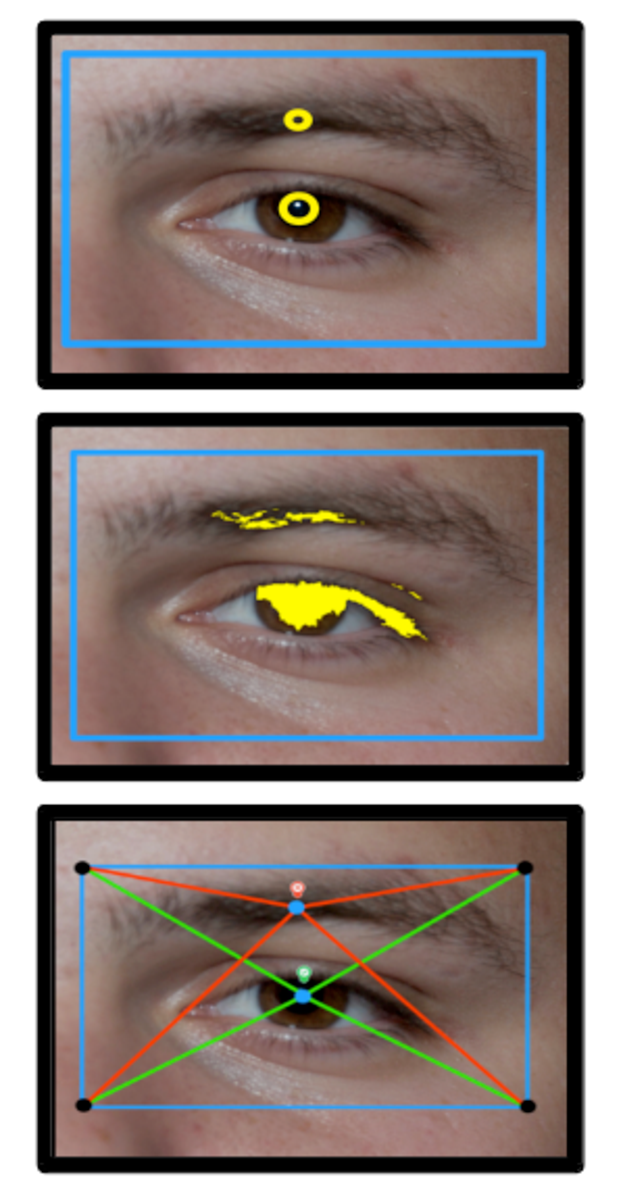
\includegraphics[width=2.5in]{figs/pupilDetection.pdf}

    \caption{Pupil Detection Process}

\end{figure}

Detecting the pupils enables $\Name$ to determine the gaze direction.
Pupil detection in this approach is aimed to be fast in order to be deployable
onto web frameworks. Firstly, the frame is converted to grayscale and the eye
is detected using the Viola-Jones Object Detection Framework \cite{Viola01}.
The region of interest (ROI) is then thresholded for an array of different
shades. Connected components are then detected on these binary images. All of
the detected connected components are stored as possible pupils.  Out of these
possible pupils, the one with the minimum overall error is designated as the
pupil.  Below are the expressions to be minimized.

\begin{eqnarray}
\Function{err}_{\alpha}(p) &=& \frac{
    \mathlarger{\sum}_{c \in Corners}{
        \vert
            \frac{\pi}{4} - \Function{arctan}(
                \vert \frac{p_y - c_y}{p_x - c_x} \vert
            )
        \vert
    } }{\pi} \\ \Function{err}_{size}(p) &=& \frac{ \vert \Var{avgPupilSize} -
    \Function{size}(p) \vert }{2} \end{eqnarray}

$\Function{err}_{\alpha}$ refers to how far the center of the connected
component is from the center of the Haar bounding rectangle. We use angle
deviation instead of pixel distance for this metric because we assume that the
pupil would not always reside immediately in the center of the boundary
rectangle. A direct pixel distance might yield other connected components more
suitable.  The angle deviation acts a weak error function in order to be more
lenient without the use of constants.  Once the connected component with the
minimum error is extracted, its center is returned.

$\Function{err}_{size}$ refers to the difference between the scaled area of the
detected blob and the average scaled area of a general pupil. This means that
during the thresholding process, out of the  array of connected components
detected with minimal $\Function{err}_{\alpha}$, the one that has the area
closest to that of an average pupil will be returned.

Using a combination of these two error functions, we are able to detect the
pupils accurately and derive a gaze metric.

\textbf{Figure 1} depicts the process of pupil detection. The photo on the top
left shows the connected component segmentation. In the top right image, the
centers of the connected components are extracted. The image on the bottom left
shows that out of the two detected connected components, the one with the green
lines has a smaller overall error and is returned as the pupil. 

\subsection{Determining the Gaze Metric}

The gaze metric is a quantifiable measurement that describes the gaze direction
for an eye. To determine the gaze direction, we must be able to capture the
movement of the pupil relative to the eye position. This is done by computing
the horizontal and vertical displacements from the center of the Haar bounding
rectangle surrounding the eye to the pupil center. Since the center of the Haar
bounding rectangle stays in a constant position with reference to the pupil, it
can be used to discern the relative movment of the pupil.

Using a point that remains in a relatively constant position with reference to
the pupil is vital for determining the gaze direction because the determined
gaze will not be affected by the movment of the head or the jitter of the
camera.

\begin{figure}[ht]

    \centering

    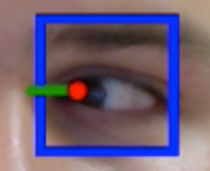
\includegraphics[width=1.3in]{figs/gazePrediction.pdf}

    \caption{Determining the Gaze Metric}

\end{figure}

 Since the gaze metric is represents pupil's displacement from the center, it
 can be represented as a 2D vector. In \textbf{Figure 2}, this vector is being
 drawn from the pupil center. This gives us a visual representation of the gaze
 direction. This metric is also used in calibration so that we can interpolate
 the position on the screen that user is looking.

\subsection{Calibration}

Calibration in an eye tracking system is necessary to ensure that the predicted
point of gaze resembles the expected point of gaze. The calibration creates a
mapping from what the eye tracker determines the gaze metric is to a point on
the screen. For visible light based eye tracking using commodity eye trackers,
neural network \cite{holland2012eye} and linear based calibration techniques
have been deployed. In our work, we use a linear based approach due to ease of
implementation and computing power restrictions imposed by doing the
computation inside the browser in real-time.

The linear approach works by placing sample points in the corners of the
viewing screen and asking the user to look at these points, one at a time.
Using the data gathered from the eye tracker and the knowledge of what point
the data corresponds to on the screen, we can construct a linear mapping from
the gaze metric onto the screen. We map the distance from the \emph{preceived}
point on the top left to the preceived point on the top right to the width of
the screen. We also map the distance from the preceived top left point to the
preceived bottom right point to the height of the screen. This mapping build
parametric equations that be used to interpolate the looking point on the
screen.

The user basically creates a box in which the eye tracker thinks its looking in
and maps the height and width of this preceived box to the dimensions of the
screen.

The application we created for calibration presents a point in each corner of
the screen one at a time. The user is told to look at the given point click on
the screen when they are done. The click on the screen will show each
calibration point until all of the corners have been mapped.

\subsection{Obtaining Video Data}

%\begin{figure}[ht]
%
%    \centering
%
%    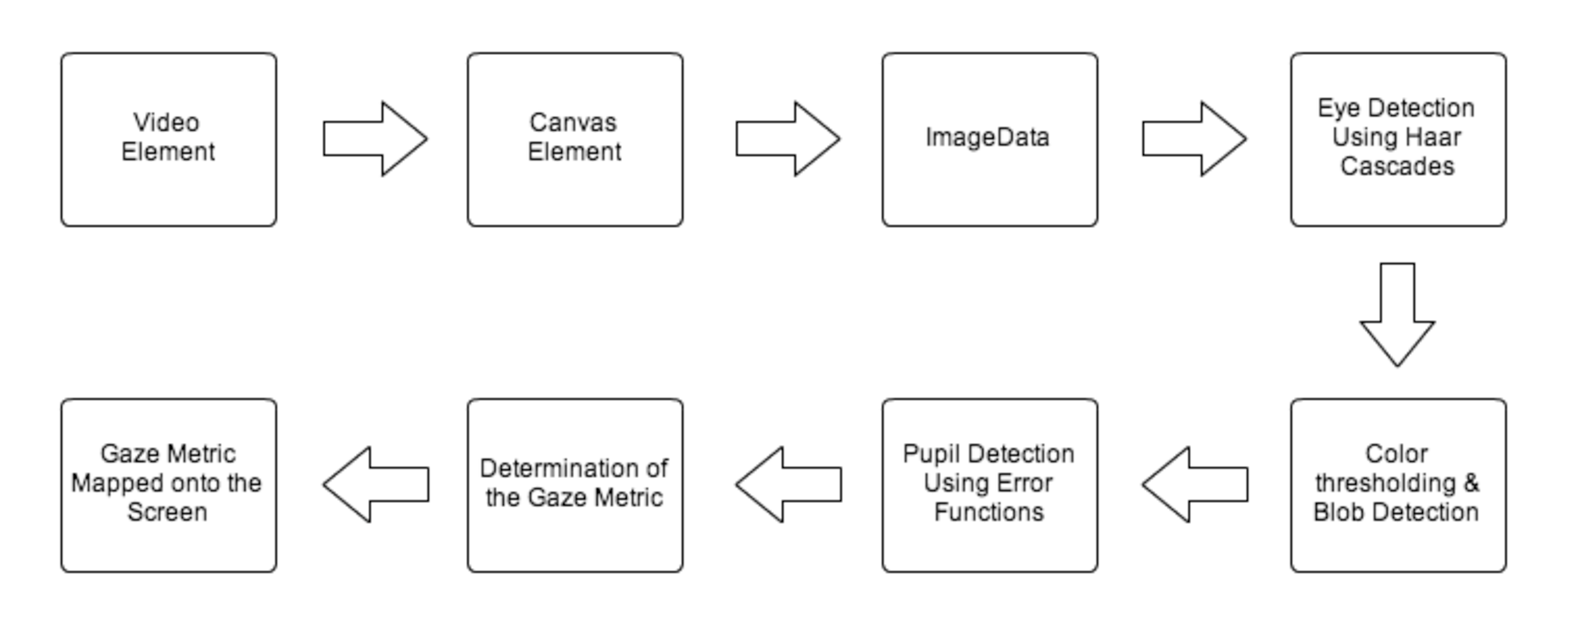
\includegraphics[width=3in, height=2in]{figs/Camgaze.pdf}
%    \caption{Structure of Camgaze.js Implementation}
%
%\end{figure}

Due to constraints imposed by JavaScript as a language while writing computer
vision applications, there are certain steps that need to be taken when
implementing the algorithms described above. Firstly, a video tag needs to be
already present in the HTML or created by the JavaScript application in order
for a video feed to be retrieved from the camera. Likewise, a canvas element
needs to be present in the HTML in order to retrieve the RGBA pixel values for
the video.  This is because the video element needs to be drawn onto the canvas
in order to retrieve the $\Acronym{ImageData}$ object for it. Once the
$\Acronym{ImageData}$ has been obtained, processing mentioned above can take
place.

\section{Methodology}

\section{Results}

\section{Discussion}

\subsection{Privacy Concerns}

$\Name$ has an ambition of bringing eye tracking to larger-scale deployment.
This intensifies the need to address the privacy concerns some users might
have. The library we describe attempts to do this in several ways.

When the user accesses a web page that uses $\Name$, they are prompted a
notice that the website is attempting to use the video from their computer.
This is the default behaviour of both Chrome and Firefox and this behaviour can
not be overridden by any website. $\Name$ displays a notice, disclosing for
what specific purposes this data will be used. Thus, we prevent capturing the
data from unaware user.

As previously mentioned, $\Name$ is implemented in Javascript. Since the
absolute majority of modern web browsers have an built-in Javascript
interpreter, it is possible to do the eye tracking on the client-side. This
allows the proposed solution to avoid sending and storing the user’s video
stream to an external server.

In general, we believe that sensible measures have been taken to mitigate the
impact on the user’s the privacy.

\subsection{Limitations}

\section{Future Research \& Applications}

Preliminary experiments show that $\Name$ is working on a tablet computer
(Google Nexus 7 -- 2013 version, Chrome Beta 30.0.1599.81, V8 3.20.17.13
Javascript engine), which brings a potentiall to bring eye tracking to a
variety of hanheld devices. Further research could concentrate of feasibility
of eye tracking on even smaller devices -- smartphones and “phablets” (phones
with a screen wider than 5’ inches).

We hope to make progress with porting one of the popular Computer Vision
libraries to Javascript, thus allowing to apply the latest developments in the
field for the task that $\Name$ tries to solve.

Additional research on the normalization of the video stream could be done.
Porting some of the algorithms to Javascript would be a novel task. 

We believe that $\Name$ should be used in cases, where the simplicity and
scalability of deployment overweights the need for perfect precision of point
of gaze prediction. Ability to open a webpage, click “ok” on a pop-up bar, and
start eye tracking opens up possibilities for use of eye tracking for various
new applications, which were previously “solvable” by eye tracking, but never
were able to get applied outside the controlled lab environment.

For example, Heitger et al. has shown that impaired eye movements in
post-concussion syndrome patients indicate trauma on the brain that surpasses
the influence intellectual ability \cite{Heitger2009}. The use of current
generation eye tracking hardware / software combinations makes a deployable
solution for testing concussions based eye movements difficult. $\Name$ has the
ability to be used in these deployable senarios such as Emergency Rooms,
abulances, and sports centers.

\bibliographystyle{acmsiggraph}
\bibliography{paper}

\end{document}
